%=======================================================================================%
% the main points of this introduction are 
% outline the complexity of biological systems for physicists
% 	> even though our theoretical models should preidct everything on the energy and length scales of biology we can't because of their heterogeneity.
%   > Give examples of the heterogenaity 
% Give some points on the history of molecular biophysics  
%   >  Hodgkin-Huxley Models
%   > Gramicidin 
% Point out how Cystic Fibrosis is an expression of this progression, going from genotype to phenotype using an ion channel to teach us biophysics. 
% conclusion.
\pagenumbering{arabic}
\chapter*{Foreword}
\setcounter{page}{1}
\label{chap:foreward}
\chapquote{} {}
\vspace
The past few years I have been captivated by the fabulous complexity exhibited by biological systems. The mindset for solving biological problems feels very different to the focus we cultivate in students when they study idealised problems in mathematics and physics. The problems are broader, and many hands are needed to solve them. Note that all the publications arising from this thesis have many many authors. Each researcher specialises like their cells.

The more I wrote this thesis the more I found myself writing for my past self, so I think this thesis will be best read by my future students. A second year grasp of physics should be sufficient to digest all of the contents herein, as the tone is quite pedagogical and the mathematics is light. What will be less familiar to these students is the breadth of pre requisits to understand teh contents. What I have not had time to do is write an introduction to molecular biology, so there may be much chemistry missed by my students. So I reccomend a physics based introduction to those concepts such as those found in \cite{phillips2012}. On this note of pedagogy, care is taken to name certain authors to give the reader a kind of anchor for where to look in the literature.  

If the reader is anything like myself they will find the amount of up front knowledge to discover in biology daunting. It is quite difficult at first to figure out what questions to ask or even which subfield a question belongs to. Such issues are best alleviated by cultivating a broad coallition of connections, speak to medical doctors, clinicians, molecular biologists, cell biologists, biochemists, computer scientists, neuroscientists, physicists, mathematicians, everyone. It will take time but remain patient and you will quickly find that a physics based approach can indeed explain and often evne predict outcomes in biological experiments.

An extensive review of the literature in the introductory chapter \ref{chap:introduction} and \ref{chap:methods} will hopefully serve as a road map for my future students. The issue is that the field is now progressing so quickly that I'm sure much of this thesis will be out of date by the time I've given it to a student to read. In a rapidly evolving field like this I think my advice would be to seek out members of the biophysics community and continue to collaborate

The heterogeneity of biology is easy to observe. If you look at your arm, you will notice hair, pores, dry skin, dead skin, perhaps even tendons and muscles twitching beneath the surface. If you were to take a single cell from just beneath the skin and stain it to distinguish features in an electron microscope, you would find all sorts of complex structures called organelles. The size, shape and function of these elements would be different if the cell was taken from somewhere else in your body. Within and between each those organelles is a salty, wet dance of molecules large and small. This journey from your arm to your organelles spans 5 orders of magnitude. The complexity across length scales hints at the reasons behind biology's physical complexity. Plasma physicists may use the same mathematical tools to describe materials as diverse as the dense stellar core to the sparse intergalactic nebulae these span 28 orders of magnitude in density \cite{chen2018}. Would that we were so lucky in biology where we struggle to apply same physical models to deal with phenomena across a single order of magnitude.  


\begin{figure}
	\begin{center}
		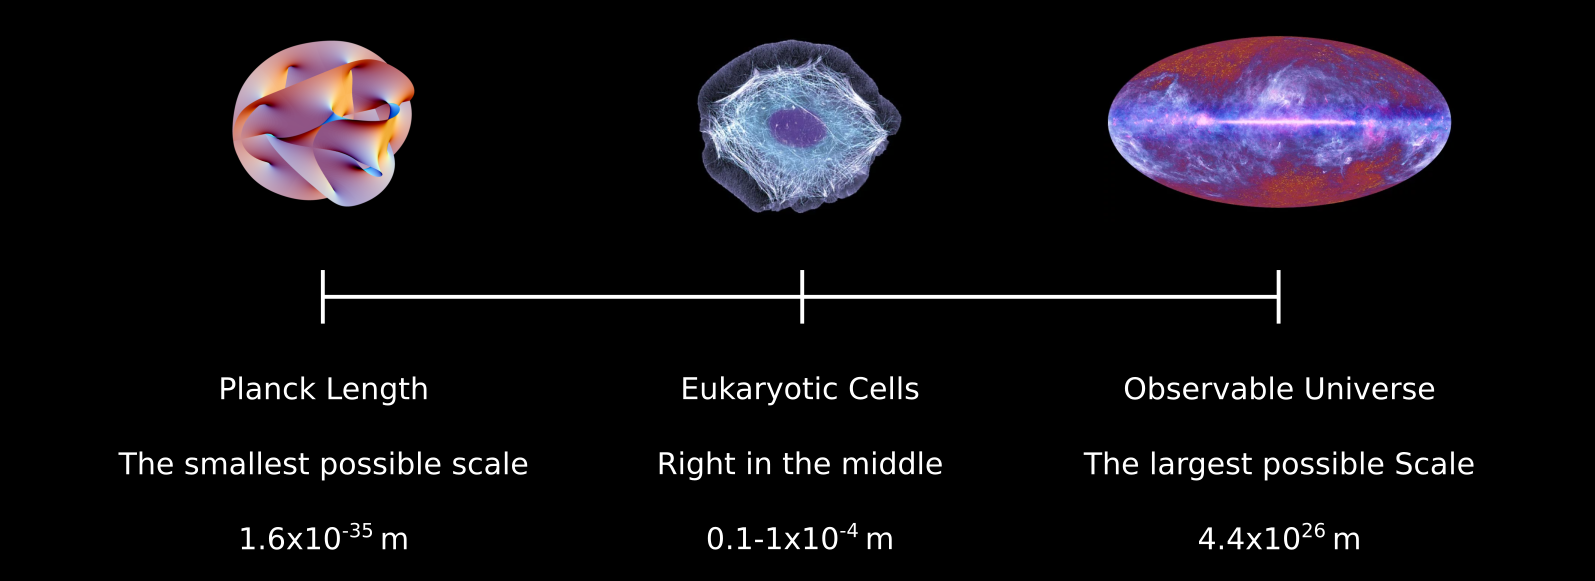
\includegraphics[width=1.0\textwidth]{figures/scales.png}
	\end{center}
	\captionsetup{singlelinecheck = false, justification=raggedright}
	\caption[The strange position that biological phenomenon occupy compared to the rest of physics] {\textbf{The strange position that biological phenomenon occupy compared to the rest of physics}}{It just so happens that if you plot the size of everything  in the universe on a log scale, eukaryotic cells fall right in the middle. A physicist can talk about both ends of this scale, we should learn something about the middle too.}
	\label{biology_scales}
\end{figure}

